%!TEX root = ../../master.tex
\section{Monolithic Architecture}
The term \textit{monolithic} was used to describe software applications that grow into monoliths by Raymond in 2003.

\begin{citat} []
"Many programmers with excellent judgment about how to break up code into subroutines nevertheless wind up writing whole applications as monster single-process monoliths that founder on their own internal complexity" \textbf{Raymond, 2003} \cite[p. 188]{raymond2003taoup}.
\end{citat}

\noindent
The word \textit{monolith} originates from Greek and means \textit{single stone}. In software, this corresponds to using a single process instead of splitting services into multiple processes that each does one thing well. Splitting services into several processes is used extensively in microservice architecture which is why monolithic architectures often are used to describe the opposite. \\

\noindent
In a monolithic architecture, all functionality of the application is packaged together as a single unit. This single unit can e.g. be a JAR or WAR file for Java applications. Monolithic architecture style is described by Lewis and Fowler as: \textit{"The server-side monolithic application will handle HTTP requests, execute domain logic, retrieve and update data from the database, and select and populate HTML view to be sent to the browser"} \cite[p. 2]{lewis2014nutshell}. Communication between components is accomplished through intra-process method invocations. Villamizar et al describe monolithic applications: \textit{"In monolithic applications all services are developed on a single codebase shared among multiple developers, when these developers want to add or change services they must guarantee that all other services continue working"} \cite[p. 584]{villamizar2015evaluating}. The benefit of easily communicating between components has the drawback of complexity for e.g. enterprise developer teams.

\begin{figure}[H]
    \centering
    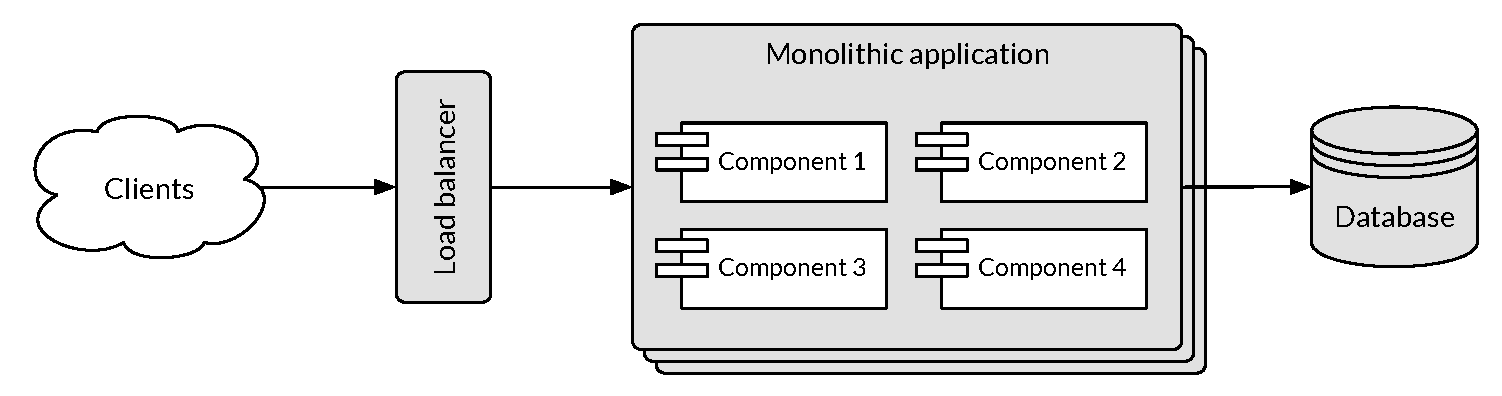
\includegraphics[width=12cm]{figures/monolithic_architecture}
    \caption{Monolithic Architecture}
    \label{fig:monolithic}
\end{figure}

\noindent
Running a single instance of a monolithic application is easy, and mapping between one application and one running process is easy to understand. The simplicity, though, comes at the price of scalability regarding the ability to innovate rapidly and scale computing resources efficiently. Scaling a monolithic architecture leads to duplicates of the entire application (Figure~\ref{fig:monolithic}). Even though only one of the components is stressed, all of the components scale up which can lead to wasted resources. \\

\noindent
Gupta states some of the advantages of a monolithic architecture as: well known, IDE-friendly, easy sharing, simplified testing, and easy deployment \cite{arongupta}. Monolithic architectures are widespread, and developers are schooled to work in such environments. IDEs such as Visual Studio, eclipse, and IntelliJ IDEA are built around solutions and projects that easily can grow big. Testing is easy since everything is in one place. Even though there are many benefits of applying the monolithic application architecture, at some point it will evolve into what Gupta refers to as a \textit{big ball of mud}. This happens over time, when teams grow, when experienced developers leave and new ones join, and when there is a constant pressure to deliver. Gupta describes the following disadvantages of a monolithic architecture as: limited agility, an obstacle for continuous delivery, "stuck" with technology stack, and technical debt \cite{arongupta}. Limited agility refers to the deployment the monolith in its entirety every time a change is made. Over time monoliths will grow and build times will get long and slow, and therefore become an obstacle for continuous delivery. The choice of technology happens before the process of building the application begins. This results in a "technology lock-down" that can require a rewrite of the entire application to break out of.